\chapter{Preliminaries}
\label{chap:preliminaries}
Throughout this thesis we will develop a complicated algorithm. We will rely on existing technology and knowledge throughout the third and the fourth chapter. Thus, in this chapter we present a minimal mindset that is helpful to understand the presented algorithm and reproduce our argumentation. \\
First, we will present in \nameref{sec:RelatedWork} what others did to solve problems similar to ours.
Then we will provide a little background knowledge on the computability of different specializations of the constraint satisfaction problem and the algorithms that are applied to the considered problems in \nameref{sec:Maths}. 
`\textbf{A} \textbf{M}athematical \textbf{P}rogramming \textbf{L}anguage' (AMPL) is used in the presented algorithm; thus, we will explain the basic concepts of AMPL in \nameref{sec:AMPL}. 
% TODO make damn shor UML Section
% The second technology we need prior knowledge about is the \textbf{U}nified \textbf{M}odelling \textbf{L}anguage (UML) and the \textbf{O}bject \textbf{C}onstraint \textbf{L}anguage, since those are the input languages for the presented algorithm.
%Further it is also necessary to shortly elaborate on the taxonomy in the field of Model--Based Testing to avoid confusions. 
\section{Literature Review}
\label{sec:RelatedWork}
\begin{figure}
\begin{center}
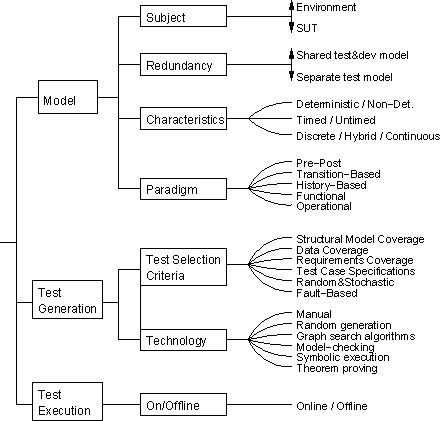
\includegraphics[width=0.6\textwidth]{./pics/taxonomyOfMBT.pdf}
\end{center}
\caption{Overview of the Taxonomy of Model-Based Testing by Mark Utting \cite{utting2006taxonomy}}
\label{fig:UttingTaxonomy}
\end{figure}
Model--Based Testing emerged in the 1990s. A variety of different modelling paradigms and languages as well as test generation methods have been proposed since then. Model--Based Testing has also been applied in different scopes, such as, for unit testing or system testing. Mark Utting offers in \cite{utting2006taxonomy} a possible classification of approaches to Model--Based Testing in seven orthogonal dimensions. In Figure \ref{fig:UttingTaxonomy}, we see an overview of possible categorisations of Model--Based Testing approaches. Any work on Model--Based Testing roughly consists of three important steps: Specifying what the test model is, generating some abstract representation of test cases, and refining the abstract test cases into concrete executable test cases by determining the necessary input data and potentially also providing an oracle value for the expected output. The rest of this section is structured according to those three steps and in each subsection we will shortly present the propositions made in different publications and use Mark Utting's taxonomy to classify them and to position our own thesis relative to them.
%in we will present  refer to several other publications and position our own thesis. The rest of this section is organized just 
% 
%  that means telling whether it models the behaviour of the SUT or whether it models its environment e.g. typical use cases. Usually a system is build according to a specification the specification can be formalized in a model from which can serve as a common source for implementation and test generation or there is a separate model for both purposes. and also the tests are derived from the specification.  with the help of the taxonomy proposed by M. Utting.
\subsection{Test Models}
In \cite{lackner2012modeling} Lackner and Schlingloff propose to build a test model independently from the implementation. Their test models modelled the behaviour of the system. They present three transition--based modelling paradigms suitable for automated test case generation: Abstract State Machines, UML2 State Machines, and Timed Automata. Early research on Model--Based Testing performed by A. Abdurazik and Jeff Offutt \cite{Offutt99GeneratingTestsFromUmlSpec} also proposed using UML state charts as test model to generate system level test cases from them. The same authors proposed in \cite{Abdurazik00usingumlCollaborationTestGeneration} UML collaboration diagrams as test models. Stephan Wei{\ss}leder and Dehla Sokenou propose in \cite{weissleder2008automatic} using UML state models together with UML class models, and OCL pre-- and post--conditions as test models.\\
It is very common to use state machines as the test model, while less research is performed on generating unit tests from UML activity diagrams. Wang Linzhang et al. propose in \cite{Linzhang04GeneratingTestCasefromActivityGrayBoxMethod} using UML activity diagrams. They propose to generate test cases from an Activity modelling an operation in the design model. They also claim to have implemented a proof--of--concept tool called UMLTGF, which, unfortunately, was unavailable for review. %Another proposal using UML Activities as test model comes from Chen Minsong et al. \cite{mingsong2006automatic}. They propose using an activity diagram to automate the selection of a subset from a set of randomly generated unit tests for a set of Java classes and methods. 
In \cite{kundu2009novel} Debasish Kundu and Debasis Samanta consider UML activity diagrams specifying use cases of the system under test.% Further work on generating test cases from activity diagrams has been performed by \cite{Patel12TestCaseFormationUsigUMLActivityDiagram}.
\\
Achim D. Bruckner and Burkhard Wolff propose in \cite{brucker2012theoremProverBasedTesting} a full theorem prover and constraint solver based approach to test generation. Thus, their input models are entered by means of a functional programming paradigm. They consider models of the system under test as well as additional information about how the system shall be tested as test model.\\
For our own work we use as test model some details from the UML class model and an UML activity diagram modelling the inner workings of the unit under test. The unit under test is in our case a C function. The model we use for test generation shares its control flow structure with the model used to generate the implementation similar to \cite{Linzhang04GeneratingTestCasefromActivityGrayBoxMethod}. The information needed to be able to derive test data is added separately to the test model, not shared with the design model, in the form of OCL pre-- and post--conditions and guards. The use of OCL constraints is similar to the work of Stephan Wei{\ss}leder and Dehla Sokenou \cite{weissleder2008automatic}. Furthermore, our input models are deterministic, untimed, and discrete. % Then they select among the randomly generated unit tests a set of unit tests whose execution traces correspond to a certain set of control flow paths from an activity diagram.
%\
% Our test models model one function of the SUT and we use a common model for development and test generation. thus the scope of our approach is unit testing  And 
\subsection{Test Generation}
In test generation, coverage criteria are a widely accepted means to measure the quality of a test suite and steer the test generation. Aynur Abdurazik and Jeff Offutt proposed in \cite{Offutt99GeneratingTestsFromUmlSpec} a handfull of coverage criteria concerned with the structure of the test model. By structure we mean the nodes and the arcs of the state chart they used as input. They present path search algorithms to find transitions sequences fulfilling the proposed coverage criteria.
%Further 3 mor sophisticated covera
%Among others they proposed transition coverage, that means the set of generated test cases should at least trigger each transition in the test model once. They also presented full sequence coverage, which basically means that every possible transition sequence in a state chart shall be satisfied by one test case which is in general impossible, since a state chart with loops contains infinitely many 
Puneet E. Patel and Nitin N. Patil compare in \cite{Patel12TestCaseFormationUsigUMLActivityDiagram} two different path finding algorithm selecting control flow paths within an activity diagram as abstract test cases. Similarly, \cite{kundu2009novel} and \cite{Linzhang04GeneratingTestCasefromActivityGrayBoxMethod} propose a kind of graph search as technology to find suitable test cases.\\
%finding a paths to select test cases in a way that they fulfil some coverage of arcs or arc sequences and nodes in an activity diagram. This is also a structural coverage criterion. 
%The coverage criterion of 
Stephan Wei{\ss}leder and Dehla Sokenou presented in \cite{weissleder2008automatic} a data oriented approach to select test cases. They propose to use abstract interpretation to derive partitions of the domain of input values. They then propose to select values at the boundaries of the computed partitions as test data.
In Stephan Wei{\ss}leders Ph.D Thesis \cite{ParTeG} we found the most detailed and complete collection of different model--structure and data--oriented coverage criteria. Furthermore, a formal definition of the coverage criteria is given. The source code of ParTeG, the proof--of--concept tool associated with this thesis, is freely available and we were able to test it. It uses graph search in combination with abstract interpretation and a comprehensive framework allowing the user to steer which coverage criteria the generated test cases will adhere to.\\
A comprehensive approach to automated test generation based on automated theorem proving and constraint solving is presented by Achim D. Brucker and Burkhart Wolff in \cite{brucker2012theoremProverBasedTesting}. They generate test cases by applying natural deduction to a test case specification given in the input language of a theorem prover. The so called test theorem resulting from the natural deduction is a sequence of executable statements that serves as abstract test case. With constraint solving concrete test data is computed for each abstract test case.\\
In our thesis we use an easy to implement path search algorithm to generate abstract test cases. The path search is supported by symbolic execution and constraint solving to determine infeasible paths.
%Among other all those publications presented the model structure oriented full sequence/path coverage, which basically means that every possible arc sequence in a graph shall be satisfied by one test case. We use a slight relaxation of this coverage criterion for our thesis. Furthermore we will also hint how we can satisfy data oriented coverage criteria.\\
% 
\subsection{Test Data Generation}
Chen Minsong et al. \cite{mingsong2006automatic} combine random test case and data generation with graph structure oriented coverage criteria. Their approach is to generate random executable unit tests for a Java implementation and matching the execution traces of the randomly generated unit tests with the control flow paths found in an activity diagram. They then select a subset from the test cases, which covers all simple paths in the test model. A simple path is a control flow path without cycles. This is a randomised approach to test data generation combined with a structural model coverage criterion.
Jan Peleska et al. \cite{peleska2011automated} describe a combination of abstract interpretation with constraint solving using an SMT solver in order to generate test data. They consider the execution of a test model as consecutive execution of a state transition function, which changes the state of the system. They have the iterated state transition function and further predicates solved by an SMT solver and support the solver by providing it with bounds for some variables deduced via abstract interpretation.\\
Using OCL as input and trying to obtain test data by solving OCL constraints there have been several proposals on how exactly to find models making an OCL formula true. Shaukat Ali et al. proposed in \cite{ali2011search} using evolutionary or genetic algorithms to search for potential solutions of OCL constraints. Matthias P. Krieger and Alexander Knapp proposed in \cite{krieger2008executingUnderspecifiedOCL} using a SAT solver to find instantiations of variables fulfilling OCL constraints. They suppose to transform OCL formulas into boolean formulas with bounded quantifiers and uninterpreted functions. Consequently they use a model finder, based on a SAT solver, capable of handling those formulas to find assignments to the variables.\\
In \cite{malburg2011combining} Jan Malburg and Gordon Fraser propose a hybrid approach. On the top level they use a genetic algorithm evolving a population of candidate test data internally they provide guidance to the genetic algorithm by providing a special mutation operator performing dynamic symbolic execution. Also the white--box unit test tool PEX \cite{pex} from Microsoft\textsuperscript{\textregistered} research is based on dynamic symbolic execution. Both publications, \cite{malburg2011combining} and \cite{pex}, propose to execute the implementation with random input values and generate new input values by collecting all path conditions along the executed control flow. Then they negate one of the path conditions and use a constraint solver to find a solution for the new constraint system. The generated solution is new input data which is guaranteed to take another control flow path in the program.\\
Our own test data generation approach is based on symbolic execution of control flow paths in an activity diagram and constraint solving using a collection of solvers through a common interface. We collect all the constraints along a control flow path and represent them in a constraint satisfaction problem which is solved by a constraint solver.
%Alloy \cite{jackson2002alloy} and Dresden OCL or Eclipse OCL are other projects that aim at executing or at least evaluating OCL specifications over a given model.
% performs 
%Many papers suppose the use of state of the art SMT solvers such as HOL or CVC to solve OCL post--conditions, pre--conditions and of operations and invariants embedded to get possible input values for functions that can be used as 
%But solving OCL constraints as a CSP is only one part of generating test data from a UML Behaviour.
%Technology Model Checking. \cite{Xu09ModelCheckingUMLActivityDiagramsFDR}. 
% \subsection{Further Readings}
% Can intuition become rigorous \cite{Aleman00CanIntuitionBecomeRigorous?}
% RoclET \cite{jeanneret2006roclet}
% OCL Modularisation \cite{akehurst2007ocl}
% 
% \subsection{Existing Tools for Automated Test Generation}
% The only tool directly targeted at generating Unit Tests form A UML specification with OCL constraints that was freely available was ParTeG by Stephan Wei{\ss}leder. In his PhD thesis Stephan Wei{\ss}leder describes a framework for applying different control flow based as well as partition based coverage criteria to state machines. He also develops a theory how all those coverage criteria are interconnected and can be simulated by each other and a transformed version of the original Test Model\cite{ParTeG}.
% 
% Spex
% 
% tell about other test generating tools (commercial, published in Papers) and ParTeG as the only one where the source code is available.\cite{ParTeG}

\section{Mathematical Foundations}
\label{sec:Maths}
\begin{figure}
\begin{center}
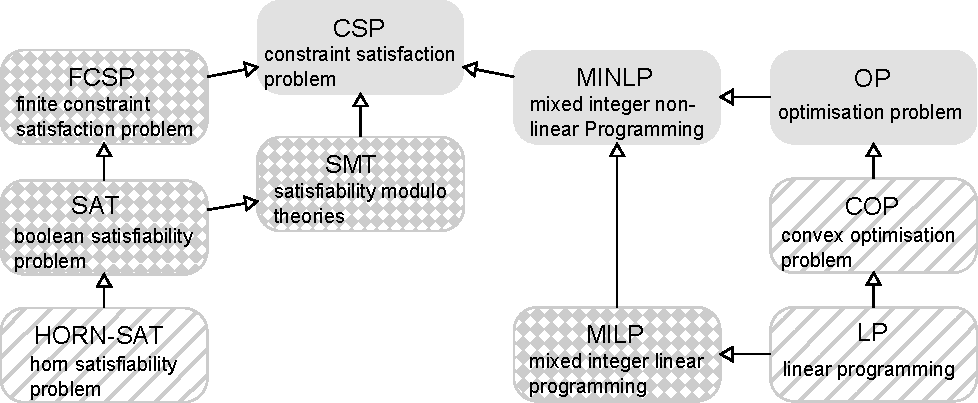
\includegraphics[width=\textwidth]{./pics/ProblemLatice.pdf}
\end{center}
\caption{Generalisation and specialization dependencies between different problems. Decidable problems for which tractable algorithms exist have a lined background; decidable problems that are NP--complete have a squared background; undecidable problems have a grey background.}
\label{fig:problemLatice}
\end{figure}
%When modelling we always need ways to express facts in mathematical terms. E.g from physic we know equations that express the relations between different physical values. 
Constraint solving is a common technique to derive answers to particular questions. Depending on the constraint satisfaction problem instance there might exist an algorithm and even a software implementation that can compute the answer to our question. A major task in this thesis is to transform a control flow path in an activity diagram into a mathematical program, that is, a constraint satisfaction problem, and to apply a constraint solver. 
\\
Depending on the used test model the resulting mathematical program will be an instance of one of the problems presented in this section. Since currently existing solvers are always specialized on particular problems one needs to understand of which problem this mathematical program is an instance. Certain problems are a specialization of more general problems. In Figure \ref{fig:problemLatice}, we give an overview of the problems presented in this Section and visualise which problems are generalisations or specializations of each other. An arrow from \textsf{A} to \textsf{B} means that \textsf{B} is a generalisation of \textsf{A}.\\
Some mathematical programs are harder to solve than others. Instances of more general problems are usually harder to solve than instances of a specialized problem. More specialized problems restrict the expressiveness of constraints that are allowed in its instances. We are especially interested in problems that allow our test models to be most expressive and are just specialized enough that we can find a useful solver for the resulting mathematical program. Those are the user--friendly problems. When we do not need the expressiveness of a general problem we can use specialized solvers computing solutions of the mathematical programs very quick. Those are the easy--to--solve problems.\\
In \nameref{sec:computability} we introduce definitions that will be used to characterise problems and methods and explain the implications of those characteristics for constraint solving. For every presented problem we will mention their characteristics. In Sections \ref{sec:MathConstraintProgramming}--\ref{sec:MathSMT} we present different means to express constraints and introduce a variety of problems. In \nameref{sec:MathSearchSpaceProperties} we will present properties of variables and introduce further problems.
\subsection{Characteristics of Problems and Solver Methods}
\label{sec:computability}
We characterise the solvers used by two orthogonal properties: the decidability of the problem they solve, and the tractability of the method they implement.
\subsubsection{Decidability of Problems}
Not every problem presented in the following subsections will be decidable. We denoted undecidable problems with a solid grey background in Figure \ref{fig:problemLatice}. 
\begin{definition}[decidability]
A problem is decidable if an algorithm solving that problem exists. 
\end{definition}
When the problem is decidable we can assume that there is an exact solver available. An exact solver will tell for a problem instance that the problem has no solution only if there really is no solution. If it returns a solution we assume it is correct.\\
When a problem is undecidable, on the other hand, that means there can never be an algorithm solving all instances of this problem. 
Still, there exist heuristics that try to handle undecidable problems. A heuristic may find a solution for a given problem instance if it is lucky, or just terminate without finding a solution although one exists, or it might run forever, or even just return a wrong answer. For instances of undecidable problems a heuristic telling that there is no solution just means that this particular search was not lucky and returned answers might not be correct solutions. For example, it can return a sub--optimal point for an optimisation. In most cases the answer of a heuristic is good enough to be useful in practice. 
If a heuristic did not find a solution one could start again with different parameters for the heuristic, for example, another starting point, or one could use another solver. In practice one will run a heuristic until a certain time limit has been reached.
\subsubsection{Tractability of Algorithms and Heuristics}
Algorithms and heuristics can be tractable or intractable. 
\begin{definition}[tractability]
A method is tractable if its worst case runtime is in $\mathcal{O}(u^n)$ for a constant $n$. 
\end{definition}
For some problems like the \emph{linear programming} (LP) explained in Section \ref{sec:MathLinearProgram} there exist tractable algorithms. In Figure \ref{fig:problemLatice}, problems for which a tractable algorithm exists have a lined background. For other problems there can be instances that are NP--complete, for example, the \emph{boolean satisfiability problem} (SAT) presented in Section \ref{sec:MathBooleanSat}. Any algorithm solving an NP--complete problem will be intractable. Problems for which no tractable algorithm exists are marked with a squared background in Figure \ref{fig:problemLatice}.\\
If the algorithm or heuristic used to solve a certain problem instance is tractable, we know that we can expect an answer even for large problem instances after a moderate amount of time. For intractable algorithms the runtime might grow exponentially and therefore make it practically infeasible to compute an answer to a given problem instance. For practical problems it is often the case that an intractable algorithm or heuristic has a non--exponential average runtime. The simplex algorithm is a good example for such an algorithm. Its worst case runtime is exponential but for problems occurring in practice its runtime grows linear with the number of constraints.
\subsubsection{Further Considerations}
Among the decidable problems those with a tractable algorithm are especially easy--to--solve. Whenever it is possible to state a certain problem as an instance of such an easy--to--solve problem it is advisable to do so. If all constraints in the used test model are instances of an easy--to--solve problem, one can be sure that there is a suitable solver solving the problem correct in a moderate amount of time with respect to the size of the problem.\\
Restricting the expressiveness of constraints to decidable problems can be a strong limitation for the user, and is not strictly required for constraint solving. It is not always easy or impossible to express constraints as a problem instance of a decidable problem that can be solved by a tractable algorithm. Consequently we will also consider using solvers for decidable problems with intractable algorithms as well as solvers for undecidable problems implementing tractable and intractable heuristics. A solver is useful in practice if it has a fair chance to produce a useful answer and if it reports useful answers for practical instances in average after a moderate amount of time. 
% 
% 
%   the worst case runtime is exponential but only for some specially crafted problem instances the worst case happens.%The simplex algorithm is a good example for such an algorithm. Its worst case runtime is exponential but for problems occurring in practice its runtime grows linear with the number of constraints.
% We therefore reduce our expectations and consider those specializations, for which algorithms exist. Among the decidable specializations of a CSP those with a tractable algorithm are especially easy--to--solve. Whenever it is possible to state a certain problem as an instance of such an easy--to--solve problem one can be sure that there is a suitable solver solving the problem correct in a moderate amount of time.\\
% 
% ISo we will also consider decidable problems with intractable algorithms as well as undecidable problems with tractable and intractable heuristics. A solver is still useful in practice if the worst case runtime is exponential but only for some specially crafted problem instances the worst case happens.%The simplex algorithm is a good example for such an algorithm. Its worst case runtime is exponential but for problems occurring in practice its runtime grows linear with the number of constraints.
% For practical problems it is often the case that an intractable algorithm has a non--exponential average runtime. 
% 
% that we can find a solver that 

\subsection{Constraint Satisfaction Problem}
\label{sec:MathConstraintProgramming}
\begin{figure}
\begin{center}
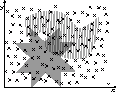
\includegraphics[width=0.5\textwidth]{./pics/SetIntersection.pdf}
\end{center}
\caption{Two--dimensional search space and three different subsets forming a constraint satisfaction problem}
\label{fig:CSPExample}
\end{figure}
In a \emph{constraint satisfaction problem} (CSP) the task is to assign values $v(x_i)$ to a set of variables $X = (x_1, \dots , x_n)$ from a \emph{search space} $S=D_1\times \dots \times D_n$ such that all relations $c_1,\dots,c_k$ between the variables hold. We call those relations $c_1,\dots,c_k$ \emph{constraints}. $D_i$ is called the \emph{domain} of $x_i$, $n$ is the number of variables, and $k$ the number of constraints. We can formalise a constraint satisfaction problem as shown in equations (\ref{CSP})--(\ref{CSPEnd}) \cite{Eiben97constraintsatisfaction}.
\begin{eqnarray} 
\label{CSP}
c_i \subseteq S \qquad\forall i \in \left[ 1 \dots k \right]\\
\text{find:} \quad v(x_i) \in D_i \qquad\forall i \in \left[ 1 \dots n \right]| \\
\label{CSPEnd}
\text{subject to:} \quad (v(x_1),\dots , v(x_n)) \in c_j\qquad\forall j \in \left[1 \dots k\right]
\end{eqnarray} 
\begin{definition}[feasible solution]
Any point in $S$ fulfilling all constraints is called a feasible solution.
\end{definition}
\begin{definition}[feasible set]
The set of all feasible solutions is called the feasible set.
\end{definition}
The feasible set is the intersection of all constraints. If the feasible set is the empty set we call the problem infeasible. Solving a constraint satisfaction problem means finding one feasible solution.\\
Practically, constraints are often specified as boolean terms over a subset of $X$. For example $x_1=x_2$ or $0\leq x_1 \leq 1$. 
% specifies a constraint. A constraint can also be specified by only one variable as in $0\leq x_1 \leq 1$.
It is possible to extend any relation between $x_1$ and $x_2$ to a n-ary relation between $x_1,\dots,x_n$. In the extended relation all possible values are permitted for the variables not contained in the term.\\
In general, there are no restrictions on the domains of the variables. They could be continuous, discrete, finite, and infinite. Well--known domains are integer, real, boolean but city names or all triangles similar to an equilateral triangle could also form a domain. Similarly, the constraints can have arbitrary properties. Even a fractal set would be acceptable as constraint.\\
In Figure \ref{fig:CSPExample}, we can see a two--dimensional continuous search space and three sets. One that could be assembled by a union of intersections of half--spaces, another that has an arbitrary shape, and the last set that consists of discrete points marked by the crosses. Any of the points within the intersection of those three sets is a solution to the corresponding CSP.\\
The CSP in its general form is undecidable but there are decidable specializations with a few restrictions on the kind of constraints and domains. For example a CSP with all variables in $\mathbb{B}$ is decidable.

%There is no way to handle all possible ways to describe the constraints by one single algorithm. Additionally this general form includes also a lot of problems that are known to be undecidable or just infeasible to compute. Consequently we need to look at several specializations. //BULLSHITT!!!!
%A constraint $c_j$ is a pair $<t_j,R_j>$ of a set of variables $t_j$ and a relation $R_j$. $t_j$ is a subset of X and R is defined over those variables.

\subsection{Optimisation Problem}
An \emph{optimisation problem} (OP) is a constraint satisfaction problem with a real--valued \emph{objective function} $f:S\mapsto \mathbb{R}$ where constraints are specified in terms of real--valued functions $g_1,\dots,g_k:S\mapsto\mathbb{R}$. We call those functions \emph{constraint functions}. The search space is $\mathbb{R}^n$. The task is to find a feasible point that minimises the objective function $f$.
\begin{eqnarray}
\text{minimise:} \quad f(X)\\
\text{subject to:} \quad g_i(X)\leq 0 \qquad \forall i\in\left[1,\dots ,k\right] \label{eqn:MOPs.t.}
\end{eqnarray}
We distinguish two kinds of optima, the local optimum and the global optimum. Global optima are in general much more difficult to find than local optima.
\begin{definition}[local optimum]
A local optimum is a feasible solution that minimises the objective function within a neighbouring set of feasible solutions.
\end{definition}
\begin{definition}[global optimum]
A global optimum is a feasible solution that gives the minimal value for the objective function among all feasible solutions.
\end{definition}
In practice equations are also used as constraints. In equation (\ref{eqn:MOPs.t.}), $\geq$ is permitted as well as an arbitrary constant on the right--hand side. \\
In this thesis only linear objective functions are considered. For linear objective functions that are not constant any optimum can be found on the boundaries of the feasible set. That is why the word \emph{boundary value} will be used as an equivalent for local optimum. Using a constant objective function relaxes the problem, since with a constant objective function every feasible point is a global optimum.\\
The OP is undecidable, but there are very successful heuristics available. One way to tackle an OP is to add quadratic penalty terms to the objective function, which are growing when a constraint is violated. Then one selects an arbitrary starting point and applies a descend method such as Newton's method to find a local minimum of the augmented objective function. One can try this local search with a descend method multiple times from different starting points and then select among the points found the one that gives the lowest value for the objective function. With a high likelihood, this algorithm will find a feasible point, and the global optimum could have been among the computed local optima.
\subsection{Convex Optimisation Problem}
\label{sec:MathCOP}
The \emph{convex optimisation problem} (COP) is a decidable specialization of the optimisation problem for which tractable algorithms exist \cite{Boyd04ConOpt}.
\begin{definition}[convex set]
A set $C$ in a vector space $S$ is said to be convex iff for all points $x$ and $y$ in $C$ and all $t\in\left[0,1\right]$, the point $(1-t)x+ty$ is in $C$.
\end{definition}
\begin{definition}[convex function]
A function f is convex iff for any two values $x$ and $y$ the inequality $ f(\theta x + (1-\theta) y)\leq \theta f(x)+(1-\theta) f(y)$ with $\theta\in \left[0,1\right] $ holds.
\end{definition}
A convex optimisation problem is an optimisation problem with a convex objective function and convex constraint functions. The intersection of convex sets is a convex set itself and the set $\left\lbrace x\in\mathbb{R}^n|g_i(x)\leq 0\right\rbrace$ is a convex set if $g_i$ is a convex function. Consequently the feasible set is also convex. For convex optimisation problems every local optimum is a global optimum.\\
The convex optimisation problem is decidable and additionally there are tractable interior point methods solving instances of that problem. Interior point methods first need a feasible point as starting point. The objective function is augmented by logarithmic barrier functions for each constraint with a form factor to steer the steepness of these barriers. Now a descend method is applied to find the lowest point. Then repeatedly the barriers are made steeper and the last point found is used as a new starting point. The repetition ends when a stop criterion is fulfilled \cite{Boyd04ConOpt}. 
\subsection{Linear Programming}
\label{sec:MathLinearProgram}
Within the class of convex optimisation problems there are many special cases. One specialization of the convex optimisation problem is \emph{linear programming} (LP).
In linear programming every constraint can be represented as linear inequality and the objective function is an affine function. 
The canonical form of a linear program consists of a matrix $\mathbf{A}$ and two vectors ${c}$ and ${b}$ as shown in the equations (\ref{linDef})-(\ref{linDefEnd}). The relation $\leq$ is evaluated componentwise.
\begin{eqnarray}
\label{linDef}
\text{minimise:}\quad {c}^TX^T \\
\label{linDefEnd}
\text{subject to:}\quad AX^T\leq{b}
\end{eqnarray}
By removing the objective function or setting ${c} = {0} $ the problem is slightly relaxed. Formulations containing also equations in the constraints on some components of $X$ can be transformed to an equivalent problem in the canonical form. Also, maximisation of the objective function might be required instead of a minimisation. Further the relation $\geq$ might replace the $\leq$ for some components of the constraint. In practice we will use all of these formulations.\\
An example of a linear program is given in equations (\ref{linExample})-(\ref{linExampleEnd}).
\begin{eqnarray}
\label{linExample}
\begin{pmatrix}
1 & -2 & 3 \\
4 & 5 & 6 
\end{pmatrix}\times\begin{pmatrix}
x_1 \\ x_2 \\ x_3
\end{pmatrix} = \begin{pmatrix}
1 \\ 4
\end{pmatrix}\\
\begin{pmatrix}
0&-1&0
\end{pmatrix}\times\begin{pmatrix}
x_1 \\ x_2 \\ x_3
\label{linExampleEnd}
\end{pmatrix}\leq \vec{0}
\end{eqnarray}
Linear programs can efficiently be solved with an implementation of the simplex algorithm \cite{dantzig63Simplex}. Although its worst case runtime is exponential the average runtime grows linearly with the number of constraints. For a geometric interpretation of the simplex algorithm we interpret the constraints as a set of hyper--planes in an $n$--dimensional space. The feasible region is a polyeder whose faces are within the hyper--planes defined by the constraints. The simplex algorithm starts at an arbitrary exposed point of this polyeder and then moves along one edge to another exposed point with a better objective value. This step is repeated until the exposed point with the minimal or maximal objective value is found.
\subsection{Boolean Satisfiability Problems}
\label{sec:MathBooleanSat}
In a classic \emph{boolean satisfiability problem} (SAT) all variables are within the boolean domain and can take the values $true$ and $false$ or $0$ and $1$ respectively. The constraint relations are expressed by a boolean formula. The task is to find an assignment to the variables that makes the formula true. A simple example of a boolean formula is given in equation (\ref{boolFormula}).
\begin{eqnarray}
x_1 \land \neg x_2  \lor \neg x_1 \land {x_2}
\label{boolFormula}
\end{eqnarray}
Any boolean formula can be normalised to a conjunction of disjunctive clauses, the so--called \emph{conjunctive normal form}. The boolean satisfiability problem is decidable, but belongs to the class of NP-complete problems. Thus, algorithms solving this problem are intractable. However, there are specializations of the SAT problem for which a solution can be computed in polynomial time, for example the \emph{horn satisfiability problem} (HORN--SAT). In HORN--SAT the boolean formulas are restricted to horn formulas. A horn formula consists of a conjunction of horn clauses. A horn clause is a disjunctive clause with at most one positive literal. A \emph{literal} can either be a variable (positive literal) or the negation of a variable (negative literal).\\
DPLL \cite{DPLL} is a classic algorithm solving the boolean satisfiability problem. The DPLL algorithm combines a backtracking search and local consistency checks. In the backtracking step one literal is selected and the problem splits up in two sub--problems, one in which the selected literal is assigned true and one, where it is set to false. All disjunctive clauses that become true by the assignment can be removed from the formula, and from those clauses that do not evaluate to true the assigned literal is removed. When there is a clause consisting of only one literal this literal can only be assigned in one way to make that clause true. In unit propagation this literal will be assigned and all clauses containing that literal can be removed from the formula. From all clauses containing the opposite literal the literal is removed. Unit propagation is repeated until there are no more clauses containing a single literal. Next, pure literals are eliminated. A pure literal is a literal that is only present with one polarity. When a variable is for example only occurring as negative literal one can assign that variable to false and all clauses containing the negative literal are evaluating to true and can be removed. If in the end there is one empty clause, that is, a clause for which all literals are assigned and evaluated to false, then the current sub--problem is not satisfiable and one has to backtrack. If there are no more clauses left that means for the current assignment of literals every clause contains at least one literal evaluating to true then a satisfying assignment for the variables has been found.
\subsection{Satisfiability Modulo Theories}
\label{sec:MathSMT}
An important generalisation of the SAT is the \emph{satisfiability modulo theories} (SMT) problem. Here, instead of literals, sentences can appear that evaluate to true or false in some theory. Common background theories used for SMT are the free theory, linear arithmetic, or the theory of bit vectors. In the equations (\ref{eqn:SMTExample})-(\ref{eqn:SMTExampleEnd}) we see an example formula containing propositions in linear arithmetic, integer arithmetic, and one boolean literal.
\begin{eqnarray}
\label{eqn:SMTExample}
x_1,x_2\in \mathbb{R}, \quad x_3 \in \mathbb{Z},\quad x_4\in \mathbb{B}\\
\label{eqn:SMTExampleEnd}
(x_1\leq 5) \land (-x_2\leq 10) \lor (x_3=2) \land x_4
\end{eqnarray}
The decidability of SMT problem formulations depends on the background theories used. If the SMT is restricted to a set of decidable background theories then the SMT is decidable. If undecidable theories such as non--linear arithmetic including transcendent functions are allowed then the SMT is undecidable. The well--known SMT solver CVC currently implements a large number of logical theories and their combinations \cite{cvc}.\\
%There are instances of SAT that are NP-complete and thus are in practice infeasible to solve although the corresponding decision problem is always decidable and DPLL is deterministic.\\
\subsection{Properties of the Search Space}
\label{sec:MathSearchSpaceProperties}
Every specialization of the CSP is imposing constraints on the formulation of constraints and on the selection of domains. For the problems presented so far, we focused on the way constraints are stated. In this section we present further problems that can be obtained by strengthening or relaxing the constraints imposed on the selection of domains.
\subsubsection{Mixed Integer Programming}
Domains can either be continuous or discrete. The optimisation problem as well as linear programming permits only continuous domains. They can be generalised by allowing variables in the discrete integer domain.\\
\emph{Mixed integer linear programming} (MILP) is a generalisation of linear programming allowing variables in the integer domain. While linear programming can be solved in polynomial time, the introduction of variables with discrete domains makes the problem NP-complete. A famous instance of this problem is the knapsack problem. In the knapsack problem it is the objective to maximise the value of undividable objects in a container where each object has a value and a weight. The sum of the weights must stay below a threshold. Mixed integer linear programming is decidable.\\
\emph{Mixed integer non--linear programming} (MINLP) is a generalisation of the optimisation problem allowing variables in the integer domain as well as the real domain. This problem contains many instances that are known to be infeasible to solve. A well--known instance is the factorisation of a number with two prime factors. Mixed integer non--linear programming is just as the optimisation problem undecidable. But while to the optimisation problem tractable heuristics similar to the algorithms for the convex optimisation problem can be applied the introduction of discrete variables also makes intractable heuristics necessary to solve mixed integer non--linear programs.
% The mixed integer linear programming contains instances that are NP complete A linear program with only discrete domains is called \emph{linear integer program} (LIP) and it is called a \emph{mixed linear integer program} (MILP) when it has both discrete and continuous domains. We call an IP or MIP whose \emph{continuous relaxation} is a convex problem a \emph{convex mixed integer program}. The continuous relaxation of a mixed integer program is the mathematical program where all discrete domains are replaced by corresponding continuous domains. For example, the set 

% \emph{Mixed}
% 
% 
% When all variables in an CSP are in the discrete domain of natural numbers we call the CSP an \emph{integer program}. Most integer programs are NP--complete.  A constraint satisfaction problem with variables in the domain of natural numbers as well in the domain of real numbers is called a \emph{mixed integer program}. The optimisation problems and linear programming can be generalised by allowing variables in the domain of natural numbers. While all linear programs with only continuous domains can be solved in polynomial time, the introduction of variables with discrete domains makes the problem much more complex. A linear program with only discrete domains is called \emph{linear integer program} (LIP) and it is called a \emph{mixed linear integer program} (MILP) when it has both discrete and continuous domains. We call an IP or MIP whose \emph{continuous relaxation} is a convex problem a \emph{convex mixed integer program}. The continuous relaxation of a mixed integer program is the mathematical program where all discrete domains are replaced by corresponding continuous domains. For example, the set 
% $\left\lbrace 1,2,3 \right\rbrace $
%  could be replaced by the interval 
%  $\left[ 1,3 \right] $
%  .\\
An instance of mixed integer non--linear programming is as follows:
\begin{eqnarray}
x_1,x_2\in \mathbb{Z},\quad x_3\in \mathbb{R}\\
\text{minimise:}\quad x_3 \\
\text{subject to:}\quad x_1^2 + x_2^2 - 10.5 + x_3 \leq 0 \\
\text{subject to:}\quad x_3 \geq 0
\end{eqnarray}
One possible solution to this problem is $x_1=1$ and $x_2=3$ and the optimal value for $x_3$ is $0.5$. Without the integral constraint on $x_1$ and $x_2$ the solution to this problem instance could be computed by an interior point method in polynomial runtime; $x_3$ would then be $0$. With $x_1,x_2\in \mathbb{N}$ one can estimate an upper and a lower bound for $x_1$ and $x_2$ and then needs to try out all combinations of possible values for those two variables.\\
To solve mixed integer linear programs a combination of different methods is used. One strategy is the cutting--planes method. For cutting--planes first the optimal solution of the \emph{continuous relaxation} is computed. The continuous relaxation of a mixed integer linear program is the linear program where all discrete domains are replaced by corresponding continuous domains. For example, the set 
 $\left\lbrace 1,2,3 \right\rbrace $
  could be replaced by the interval 
  $\left[ 1,3 \right] $
If the optimal solution is integral in all the components that are required to be an integer we are done. If that is not the case a constraint is added such that all feasible solutions are still within the new feasible set, but the currently optimal solution of the continuous relaxation is excluded. Then, the solution of the continuous relaxation of the new problem is computed. This repeats until no more additional constraint can be found or the solution is integral in those components that are required to be integral. Mathematicians have found a variety of strategies to generate those additional constraints for the cutting--planes method. Another strategy is the branch--and--bound method. In branch--and--bound, the solution of the continuous relaxation is computed first and, in case the integrality constraints are not satisfied, the problem is split into sub--problems excluding the current solution of the continuous relaxation. For example the problem above might be split up into two sub--problems, by one time adding the constraint $x_2\geq 1$ and one time adding $x_2\leq 0$ to the original problem. This separation would exclude all solutions with $x_2$ between $0$ and $1$. The solution of the continuous relaxation, however, gives a lower bound for the optimal value. An upper bound for the optimal value of a sub--problem can be gained by a heuristic. If the lower bound of sub--problem \textsf{A} is above the upper bound for sub--problem \textsf{B} then sub--problem \textsf{A} can be pruned. Thus, large portions of the search space are excluded from the search.\\
The same methods can be applied to mixed integer non--linear programming analogous. But for them it is not an algorithm but only a good working heuristic.
\subsubsection{Finite Constraint Satisfaction Problem}
When each domain is a finite set then the search space is also finite. We call a constraint satisfaction problem with finite search space a \emph{finite constraint satisfaction problem} (FCSP). In fact, on a computer, a real number is stored in IEEE 754 floating point format, which is a finite discretization of the real numbers.\\
For a \emph{finite constraint satisfaction problem} at least theoretically one can always find a solution or deny the existence of a solution after exhaustive search, thus it is decidable. In practice the search space is finite but often too large for exhaustive search.\\
%The class of mathematical programs contains instances whose decision problems are undecidable.
%In general CSPs with infinite domains and nonlinear algebraic constraints are undecidable. 
%There are some heuristic capable of solving many instances of those problems. There exist problem instances for which algorithms tend to run forever. 
%One option to break down problems with continuous or infinite search space is reducing its search space to a finite discrete set of possible values. This excludes the largest portion of the search space but makes the problem handleable with existing constraint programming systems. This technique is called \emph{bounded model checking}. The concept of bounded model checking matches pretty well with the fact that a computer can only encode finite sets. It is suitable to find a solution if there is one but if it does not find a solution it is not a guarantee that the original problem does not have a solution.
Instances of the finite constraint satisfaction problem can be solved by reducing the domains of variables by constraint propagation and checking locally for consistency and backtracking when an inconsistency is found \cite{Bessiere2006}. Constraint propagation is a kind of logical inference and based on rules for reasoning. For example from the two constraints $x\leq 5$ and $y \leq x$ one can conclude that $y\leq 5$, thus the domain of y has been reduced. Examples of working constraint logic programming systems are B-Prolog and SWI-Prolog \cite{wielemaker2011SWIProlog}.
 %A well--known bounded model checker is SMV \cite{citation needed}. 
%A different approach for solving finite constraint programs is stating the problem as an integer program and solving it with a combination of branch--and--bound and the cutting--planes algorithm.
\section{The AMPL Modelling System}
\label{sec:AMPL}
`\textbf{A} \textbf{M}athematical \textbf{P}rogramming \textbf{L}anguage' (AMPL) from Robert Fourer \cite{AMPL} is a mathematical programming language language and also a software system interfacing different solvers capable of finding valid assignments for variables in an AMPL program, that is, an instance of the constraint satisfaction problem or one of its specializations presented in Section \ref{sec:Maths}.
An AMPL program consists of two parts: the AMPL model and the AMPL data. The AMPL software system additionally provides a command language allowing the user to interact with the solver.\\
% The AMPL system accepts three kinds of input: first there is a command language telling AMPL what to do and
 
%Then AMPL has a modelling language in which different kinds of mathematical programs can be formalised. And last but not least AMPL offers a possibility to enter data for parameterised mathematical programs. 
In this section we will shortly explain the standard work flow with the command language and the concepts of the AMPL model language and the AMPL data language that are needed in this thesis.
\subsection{Command Language}
\label{sec:AMPLcommandLanguage}
When AMPL is started in interactive mode it shows a command prompt requiring the user to either enter commands or directly modify the AMPL model. When AMPL is started with an AMPL script in the command line arguments it operates in batch mode.
The normal workflow using AMPL is to load an AMPL model from a file or to enter the AMPL model directly in the console. Then one switches into the data entering mode and inputs specific values for every parameter of the loaded AMPL model or directly loads the data from a file. Now the AMPL program is ready to be solved by one of the solvers interfacing with AMPL. Therefore, we need to tell AMPL which solver shall be used and possibly set some further options. Then the \verb=solve= command is issued and AMPL will return as soon as either a solution is found, or an error has occurred, or the AMPL program has been found to be infeasible. When AMPL returns from the solve process reporting that a solution has been found, one will use the \verb=show= command to print the satisfying variable assignments.
Furthermore, AMPL provides commands to reset the currently loaded data or data and model. Commands for making on the fly modifications to the AMPL model and data without a complete reset are also available. For detailed reference of the commands the AMPL system supports, we refer to the AMPL reference manual in the appendix of \cite{AMPL}.
\subsection{Modelling Language}
The AMPL modelling language is the means used to formalise parameterised constraint satisfaction problems. 
The modelling language supports several model entities. The supported model entities relevant for our thesis are sets, parameters, variables, constraints, and objectives. Further we are using set expressions, index expressions, and arithmetic or logical expressions. We will start by explaining the expression types and then introduce the aforementioned model entities in the given order. For detailed reference we refer to \cite{AMPL}.
\subsubsection{Expressions}
\paragraph{Set and Index Expressions}
A set expression specifies a collection of values. The easiest way to specify a set is by explicitly naming each element, for example, \verb&1 2 3 4& specifies the set $\lbrace 1,2,3,4\rbrace$. A set containing a range of integers can also be specified more efficiently by stating \verb&1..4&. AMPL supports some set operations allowing one to specify the union or intersection of two set expressions.\\
Another important expression using the set expressions are index expressions. An index expression consists of an index variable and a set expression specifying the values that are assigned to the index variable one after another. Index expressions are used to iterate through a collection. An index expression in AMPL looks like \verb&{i in 0..4}& where \verb=i= is the index variable, which takes any integer value from $0$ to $4$.
\paragraph{Arithmetic, Logic, and Relation Expressions}
In AMPL arithmetic and logical expressions can be composed of a variety of arithmetic functions, constant values, variables, and parameters. AMPL has built in the basic arithmetic logical operations such as \verb=+=,\verb=-=,\verb=*=,\verb=/=,\verb=and=,\verb=or=,\verb=not= and also the exponentiation and further additional functions like \verb=sin=, \verb=cos=, \verb=if--then--else=. The set of functions available in AMPL can be extended further by loading external function libraries. The syntax of the arithmetic, logic and relation expressions in the AMPL modelling language is very intuitive. Examples of valid expressions evaluating to true or false are: \verb&x<5; a=sin(b)&; \verb&(a=5) and (not (b<=sin(c)))&. Expressions returning a numerical value are: \verb&x&; \verb&if (x<=5) then (10) else (11)&; \verb&cos(b)&; \verb&max(a,b,10)&. 
We assume the used literals \verb=x=, \verb=a=, \verb=b= and \verb=c= to be names of declared variables or parameters.
\subsubsection{Sets}
A set is a container holding a collection of values. It is declared with the keyword \verb=set=, it has a name and attributes. A set can have several dimensions, be ordered or unordered, and the default content can be specified. The content of the set can be required to be a subset of some set expression. A set expression is used to specify the elements contained in a set. The content of a set can be directly specified in the model or data section. When the content of a certain set is specified in the data then the model only contains a declaration of the set.\\
The simplest set declaration would be: \verb=set A;= just declaring a one dimensional set named \verb=A= whose contents have to be specified in the data section. 
\verb&set A within 0..4 default 1 3;& declares the set \verb=A= whose content need to be a subset of $\lbrace 0,1,2,3,4\rbrace$ and by default, when nothing else is specified in the data, the set will hold the elements 1 and 3.
% The syntax of a set declaration is 
% \begin{algorithm}
% \begin{description}
% \item[<set declaration> ::=] ``set'', <name>, <indexingExpression>, <attributes>?, ``;'' ;
% \end{description}
% \caption{EBNF of the used subset of the AMPL modelling language}
% \label{alg:OCLEBNF}
% \end{algorithm}
% The content of sets are specified via set expressions such as \verb=1..4= meaning all integers in the range from 1 to 4 or content of sets can also be specified by explicitly naming each entry or by means of set operations performed on other sets e.g. \verb&set a = b union c&. The content of a set can be included into the model, but they can also be specified in the data section, then the model would only contain a declaration of a set. The contents of the set can be required to be a subset of some set expression. For example if a set is declared as \verb&set A within 0..4;& then it would be illegal to assign the contents \verb&A= 1 5;& to the set, because $\lbrace 1, 5\rbrace$ is not a subset of $\lbrace 0,1,2,3,4\rbrace$. \\
% Any declaration in AMPL can be declared as an indexed collection of declarations. An indexing expression usually looks like \verb&{i in 0..4}& meaning that the index variable i takes all integer values from 0 to 4. Now it is also possible to declare a set \verb&set A = 1..4& and then use the indexing expression \verb&{i in A}&.
% If we now declare an indexed collection of sets such as \verb&set B {i in A} = 0..i ;& that essentially declares four sets namely B[0], B[1], B[3] and B[4] with the set B[0] containing only one element 0 and B[1] contains 0 and 1 and so on.
\subsubsection{Parameters}
A parameter holds a numerical value that can be accessed anywhere in the model. It is fixed and its value is usually specified in the data section. A basic parameter declaration looks like this: \verb=param b;=. This expression specifies a parameter b that can be used anywhere in the model. More sophisticated features of parameters will not be used in this thesis.
\subsubsection{Variables}
A variable in AMPL has an identifier and holds a numerical value. It can either be in a discrete or continuous domain, and it can have an upper and a lower bound. A variable with a continuous domain is declared by the statement: \verb=var x;=. A variable with discrete domain is declared by the statement: \verb=var x integer;=. Any model entity can be declared as an indexed collection by appending an index expression to the declaration. A variable being declared as an indexed collection of variables will look like this: \verb=var x{i in 0..4};=. This statement essentially declares 5 different variables namely \verb=x[0]=, \ldots , \verb=x[4]=. Variables can, just like parameters, be referenced anywhere in the AMPL model. When a solver is called the solver will try to assign the values of the variables in such a way that all constraints in the model evaluate to true and the objective is optimised.
\subsubsection{Constraints}
A constraint in AMPL has a name and an expression evaluating to either true or false. As already explained for variables also constraints can be declared as an indexed collection of constraints. The index variable can also be accessed inside of an indexed constraint. The declaration \verb&such that MyConstraint{i in 0..4}: x[i] <= i*b;& declares 5 constraints named myConstraint[0], \ldots, myConstraint[4]. We assume that b is the parameter and x the indexed collection of variables we have declared in the last two paragraphs. Now each of the 5 constraints refers to another index of x and imposes an upper bound on it, which also depends on the index. We could also have explicitly written out all 5 constraints.
\subsubsection{Objectives}
An objective can either be the maximisation or the minimisation of an objective function. The objective in AMPL has a name and an expression evaluating to a numerical value and specifies whether to minimise or maximise the given expression. The declaration \verb&minimize totalCost: a + b + c;& specifies that the totalCost has to be minimised and tells us that the totalCost composes from the values a, b and c which can be either variables or parameters. 
\subsection{Entering Data}
Although it is possible to specify the values of parameters as well as the elements contained in the declared sets directly in the AMPL model it is often desirable to enter them separately as data. Data can be entered in two ways either by reading them from a file or by switching into the data mode and entering it on the console. We assume that in the model the parameter \verb=b= and the set \verb=A= have been declared. Entering \verb&param b := 5;& and \verb&set A := 0 2 5;& in the data mode would set \verb=b= to 5 and set the content of \verb=A= to $\lbrace 0,2,5\rbrace$.
%\section{UML}
The Unified Modelling Language (UML \texttrademark ) is a graphical modelling language defining 13 different diagrams that can be used to describe the architecture, behaviour and interaction of a software systems. Modelling Elements of the UML are defined via the Meta Object Facility (MOF). Any Diagram is internally stored in a Machine readable fashion; this makes it suitable for more than just documentation purpose. With precise modelling a UML Model can also be executed or otherwise automatically analysed. In our case we want to use it to derive necessary test code for C-functions from their corresponding UML Activity Model. \\ We are using only a small subset of the complete UML here for this thesis. The figure \ref{relevantUMLClassDiagram} shows an overview of the most relevant UML modelling elements and their associations in a UML class diagram. We need to understand those elements and their relationships with each other. In the next chapters whenever referring to an element of the UML it will be printed in a special font such as \UMLType{Class}. When we refer to a reference element in UML we will put it into another special font for Example: \UMLReference{ownedOperations}.
\begin{figure}\label{relevantUMLClassDiagram}
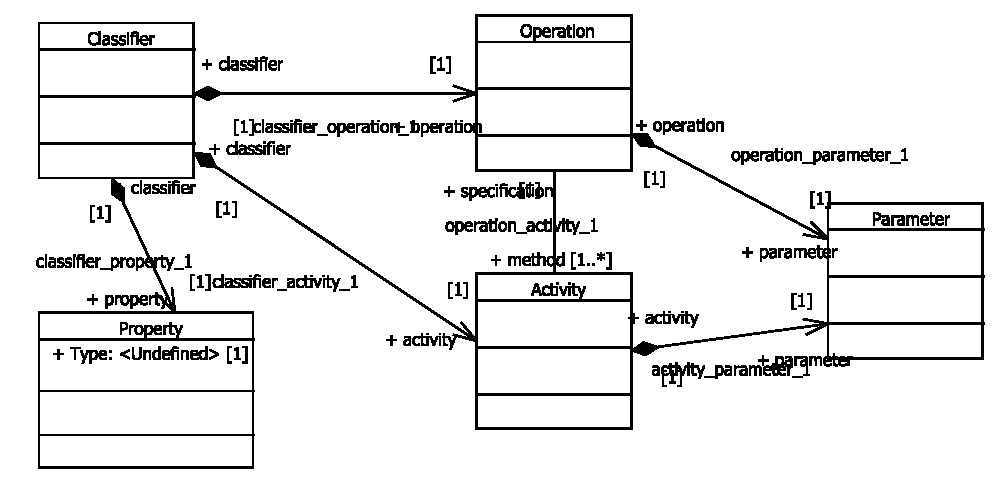
\includegraphics[width=\textwidth]{./pics/relevantUML.pdf}
\caption{Class Diagram of UML Elements used for Modelling}
\end{figure}
\subsection{Structural Modelling Elements}
\subsubsection{Package}
Packages or Namespaces are concepts that are well known to Java or C++ programmers. UML provides Packages for partitioning large Software projects. In the UML Specification we read:
\begin{quotation}
A package is used to group elements, and provides a namespace for the grouped elements.
A package is a namespace for its members, and may contain other packages. Only packageable elements can be owned
members of a package. By virtue of being a namespace, a package can import either individual members of other
packages, or all the members of other packages.
In addition a package can be merged with other packages.
\end{quotation}\cite{UML23Superstructure}
\subsubsection{Class}
The concept of classes is also pretty well known from Object Oriented Programming. In the UML specification a class is described as:
\begin{quotation}
A class describes a set of objects that share the same specifications of features, constraints, and semantics.\\
Class is a kind of classifier whose features are attributes and operations. Attributes of a class are represented by instances
of Property that are owned by the class. Some of these attributes may represent the navigable ends of binary associations.
\cite{UML23Superstructure}\end{quotation}
\subsubsection{Operation}
UML Operations are as well pretty much aligned with the wording we are used to from Object Oriented Programming. The specification says:
\begin{quotation}
An operation is a behavioral feature of a classifier that specifies the name, type, parameters, and constraints for invoking
an associated behavior.\\
An operation is invoked on an instance of the classifier for which the operation is a feature.
\end{quotation}
The associated behavior of an operation can be an Activity.
\subsubsection{Parameter} 
In programming operations, functions, procedures or methods do very often have a list of arguments or parameters. In UML they are represented by the model element Parameter.
\begin{quotation}
A parameter is a specification of an argument used to pass information into or out of an invocation of a behavioral feature. It has a type, and may have a multiplicity and an optional default value.\\
A parameter specifies how arguments are passed into or out of an invocation of a behavioral feature like an operation. The
type and multiplicity of a parameter restrict what values can be passed, how many, and whether the values are ordered.\\
...
The parameter direction specifies whether its value is passed into, out of, or both into and out of the owning behavioral
feature. A single parameter may be distinguished as a return parameter. If the behavioral feature is an operation, then the
type and multiplicity of this parameter is the same as the type and multiplicity of the operation itself.
\cite{UML23Superstructure}
\end{quotation}

\subsubsection{Constraint}
\label{sec:Constraint}
Constraints and operation contracts are modelled in UML via the modelling element \UMLType{Constraint}.
\begin{quotation}
A constraint is a condition or restriction expressed in natural language text or in a machine readable language for the
purpose of declaring some of the semantics of an element.\cite{UML23Superstructure} § 7.3.10
\end{quotation}
We exclusively consider \UMLType{Constraints} containing a textual OCL expression. How textual OCL expressions are embedded inside of a \UMLType{Constraint} is depending on the tool that is used for editing the model and modelling conventions applied by the modeller. In order not to be to restrictive we will support as many variants as possible.\\ The \UMLReference{specification} of a \UMLType{Constraint} can contain a \UMLType{LiteralString} or an \UMLType{OpaqueExpression}. How those Elements can contain textual OCL Expressions will be explained in the next two paragraphs. The OCL Language will be explained in the section \ref{sec:OCL}.
\paragraph{LiteralString}
One way to represent textual OCL in a UML Model is the model element \UMLType{LiteralString}. A \UMLType{LiteralString} contains an arbitrary string in its \UMLReference{value} attribute. Depending on the modelling convention this arbitrary string can be textual OCL.
\paragraph{OpaqueExpression}The more sophisticated way to embed textual OCL is the model element \UMLType{OpaqueExpression}. An \UMLType{OpaqueExpression} has a \UMLReference{body} and a \UMLReference{language} attribute. \UMLReference{Body} and \UMLReference{language} are multivalued string attributes. It is tool dependent how textual OCL is placed inside an \UMLType{OpaqueExpression}.\\One UML modelling tool for the Eclipse integrated development platform is Papyrus. Papyrus requires the user to put one value into the multivalued \UMLReference{language} attribute for each value specified for the multivalued \UMLReference{body}. So when the $n$-th \UMLReference{language} value is "OCL" then the $n$-th \UMLReference{body} will be a textual OCL expression.\\
The commercial tool Artisan Studio\textregistered from Atego\texttrademark will split the user supplied text for a \UMLType{Constraint} after each white-space. Each of those substrings separated by white spaces is represented as a \UMLReference{body} value of an \UMLType{OpaqueExpression}. The \UMLReference{language} attribute will be left empty.


%\begin{quotation}
%A constraint is a condition or restriction expressed in natural language text or in a machine readable language for the
%purpose of declaring some of the semantics of an element.
%\\
%Constraint contains a ValueSpecification that specifies additional semantics for one or more elements. 
%%Certain kinds of
%%constraints (such as an association “xor” constraint) are predefined in UML, others may be user-defined. 
%... A user-defined
%Constraint is described using a specified language, whose syntax and interpretation is a tool responsibility. One
%predefined language for writing constraints is OCL. 
%%In some situations, a programming language such as Java may be
%%appropriate for expressing a constraint. In other situations natural language may be used.
%Constraint is a condition (a Boolean expression) that restricts the extension of the associated element beyond what is
%imposed by the other language constructs applied to that element.\\
%
%A Constraint represents additional semantic information attached to the constrained elements. A constraint is an assertion
%that indicates a restriction that must be satisfied by a correct design of the system. The constrained elements are those
%elements required to evaluate the constraint specification. In addition, the context of the Constraint may be accessed, and
%may be used as the namespace for interpreting names used in the specification. For example, in OCL ‘self’ is used to refer
%to the context element.
%\\
%The owner of the Constraint will determine when the constraint specification is evaluated. For example, this allows an
%Operation to specify if a Constraint represents a precondition or a postcondition.\cite{UML23Superstructure}\end{quotation}

\subsection{Behavioral Modelling}
\subsubsection{Activities}
\begin{quotation}
An activity is the specification of parameterized behavior as the coordinated sequencing of subordinate units whose
individual elements are actions. There are actions that invoke activities (directly by “CallBehaviorAction (from
BasicActions)” on page 250 or indirectly as methods by “CallOperationAction (from BasicActions)” on page 252).
Generalizations
 “Behavior (from BasicBehaviors)” on page 445
Description
An activity specifies the coordination of executions of subordinate behaviors, using a control and data flow model. The
subordinate behaviors coordinated by these models may be initiated because other behaviors in the model finish
executing, because objects and data become available, or because events occur external to the flow. The flow of execution
is modeled as activity nodes connected by activity edges. A node can be the execution of a subordinate behavior, such as
an arithmetic computation, a call to an operation, or manipulation of object contents. Activity nodes also include flow-of-
control constructs, such as synchronization, decision, and concurrency control. Activities may form invocation hierarchies
invoking other activities, ultimately resolving to individual actions. In an object-oriented model, activities are usually
invoked indirectly as methods bound to operations that are directly invoked.
Activities may describe procedural computation. In this context, they are the methods corresponding to operations on
classes. Activities may be applied to organizational modeling for business process engineering and workflow. In this
context, events often originate from inside the system, such as the finishing of a task, but also from outside the system,
such as a customer call. Activities can also be used for information system modeling to specify system level processes.
Activities may contain actions of various kinds:
 Occurrences of primitive functions, such as arithmetic functions.
 Invocations of behavior, such as activities.
• Communication actions, such as sending of signals.
• Manipulations of objects, such as reading or writing attributes or associations.
324
UML Superstructure Specification, v2.3
Actions have no further decomposition in the activity containing them. However, the execution of a single action may
induce the execution of many other actions. For example, a call action invokes an operation that is implemented by an
activity containing actions that execute before the call action completes.
Most of the constructs in the Activity clause deal with various mechanisms for sequencing the flow of control and data
among the actions:
• Object flows for sequencing data produced by one node that is used by other nodes.
• Control flows for sequencing the execution of nodes.
• Control nodes to structure control and object flow. These include decisions and merges to model contingency. These
also include initial and final nodes for starting and ending flows. In IntermediateActivities, they include forks and joins
for creating and synchronizing concurrent subexecutions.
• Activity generalization to replace nodes and edges.
• Object nodes to represent objects and data as they flow in and out of invoked behaviors, or to represent collections of
tokens waiting to move downstream.

%\textbf{Semantics}
The semantics of activities is based on token flow. By flow, we mean that the execution of one node affects, and is
affected by, the execution of other nodes, and such dependencies are represented by edges in the activity diagram. A token
contains an object, datum, or locus of control, and is present in the activity diagram at a particular node. Each token is
distinct from any other, even if it contains the same value as another. A node may begin execution when specified
conditions on its input tokens are satisfied; the conditions depend on the kind of node. When a node begins execution,
tokens are accepted from some or all of its input edges and a token is placed on the node. When a node completes
execution, a token is removed from the node and tokens are offered to some or all of its output edges. See later in this sub
clause for more about how tokens are managed.
All restrictions on the relative execution order of two or more actions are explicitly constrained by flow relationships. If
two actions are not directly or indirectly ordered by flow relationships, they may execute concurrently. This does not
require parallel execution; a specific execution engine may choose to perform the executions sequentially or in parallel, as
long as any explicit ordering constraints are satisfied. In most cases, there are some flow relationships that constrain
execution order. Concurrency is supported in IntermediateActivities, but not in BasicActivities.
Activities can be parameterized, which is a capability inherited from Behavior (see 12.3.9, “ActivityParameterNode (from
BasicActivities),” on page 345). Functionality inherited from Behavior also supports the use of activities on classifiers
and as methods for behavioral features. The classifier, if any, is referred to as the context of the activity. At runtime, the
activity has access to the attributes and operations of its context object and any objects linked to the context object,
transitively. An activity that is also a method of a behavioral feature has access to the parameters of the behavioral
feature. In workflow terminology, the scope of information an activity uses is called the process-relevant data.
Implementations that have access to metadata can define parameters that accept entire activities or other parts of the user
model.

An activity with a classifier context, but that is not a method of a behavioral feature, can be invoked after the classifier is
instantiated. An activity that is a method of a behavioral feature is invoked when the behavioral feature is invoked. The
Behavior metaclass also provides parameters, which must be compatible with the behavioral feature it is a method of, if
any. Behavior also supports overriding of activities used as inherited methods. See the Behavior metaclass for more
information.
Activities can also be invoked directly by other activities rather than through the call of a behavioral feature that has an
activity as a method. This functional or monomorphic style of invocation is useful at the stage of development where
focus is on the activities to be completed and goals to be achieved. Classifiers responsible for each activity can be
assigned at a later stage by declaring behavioral features on classifiers and assigning activities as methods for these
features. For example, in business reengineering, an activity flow can be optimized independently of which departments
or positions are later assigned to handle each step. This is why activities are autonomous when they are not assigned to a
classifier.
Regardless of whether an activity is invoked through a behavioral feature or directly, inputs to the invoked activity are
supplied by an invocation action in the calling activity, which gets its inputs from incoming edges. Likewise an activity
invoked from another activity produces outputs that are delivered to an invocation action, which passes them onto its
outgoing edges. See “Parameter (from CompleteActivities)” on page 409 for more about how activities start and stop
execution.
An activity execution represents an execution of the activity. An activity execution, as a reflective object, can support
operations for managing execution, such as starting, stopping, aborting, and so on; attributes, such as how long the
process has been executing or how much it costs; and links to objects, such as the performer of the execution, who to
report completion to, or resources being used, and states of execution such as started, suspended, and so on. Used this
way activity is the modeling basis for the WfProcess interface in the OMG Workflow Management Facility,
www.omg.org/cgi-bin/doc?formal/00-05-02. It is expected that profiles will include class libraries with standard classes
that are used as root classes for activities in the user model. Vendors may define their own libraries, or support user-
defined features on activity classes.
Nodes and edges have token flow rules. Nodes control when tokens enter or leave them. Edges have rules about when a
token may be taken from the source node and moved to the target node. A token traverses an edge when it satisfies the
rules for target node, edge, and source node all at once. This means a source node can only offer tokens to the outgoing
edges, rather than force them along the edge, because the tokens may be rejected by the edge or the target node on the
other side. Multiple tokens offered to an edge at once is the same as if they were offered one at a time. Since multiple
edges can leave the same node, the same token can be offered to multiple targets. However, a token can only be accepted
at one target. This means flow semantics is highly distributed and subject to timing issues and race conditions, as is any
distributed system. There is no specification of the order in which rules are applied on the various nodes and edges in an
activity. It is the responsibility of the modeler to ensure that timing issues do not affect system goals, or that they are
eliminated from the model. Execution profiles may tighten the rules to enforce various kinds of execution semantics. Start
at ActivityEdge and ActivityNode to see the token management rules.
Tokens cannot “rest” at control nodes, such as decisions and merges, waiting to move downstream. Control nodes act as
traffic switches managing tokens as they make their way between object nodes and actions, which are the nodes where
tokens can rest for a period of time. Initial nodes are excepted from this rule.
A data token with no value in is called the null token. It can be passed along and used like any other token. For example,
an action can output a null token and a downstream decision point can test for it and branch accordingly. Null tokens
satisfy the type of all object nodes.
UML Superstructure Specification, v2.3
327
The semantics of activities is specified in terms of these token rules, but only for the purpose of describing the expected
runtime behavior. Token semantics is not intended to dictate the way activities are implemented, despite the use of the
term “execution.” They only define the sequence and conditions for behaviors to start and stop. Token rules may be
optimized in particular cases as long as the effect is the same.
Package IntermediateActivities
Activities can have multiple tokens flowing in them at any one time, if required. Special nodes called object nodes
provide and accept objects and data as they flow in and out of invoked behaviors, and may act as buffers, collecting
tokens as they wait to move downstream.
Package CompleteActivities
Each time an activity is invoked, the isSingleExecution attribute indicates whether the same execution of the activity
handles tokens for all invocations, or a separate execution of the activity is created for each invocation. For example, an
activity that models a manufacturing plant might have a parameter for an order to fill. Each time the activity is invoked,
a new order enters the flow. Since there is only one plant, one execution of the activity handles all orders. This applies
even if the behavior is a method, for example, on each order. If a single execution of the activity is used for all
invocations, the modeler must consider the interactions between the multiple streams of tokens moving through the nodes
and edges. Tokens may reach bottlenecks waiting for other tokens ahead of them to move downstream, they may overtake
each other due to variations in the execution time of invoked behaviors, and most importantly, may abort each other with
constructs such as activity final.
If a separate execution of the activity is used for each invocation, tokens from the various invocations do not interact. For
example, an activity that is the behavior of a classifier, is invoked when the classifier is instantiated, and the modeler will
usually want a separate execution of the activity for each instance of the classifier. The same is true for modeling methods
in common programming languages, which have separate stack frames for each method call. A new activity execution for
each invocation reduces token interaction, but might not eliminate it. For example, an activity may have a loop creating
tokens to be handled by the rest of the activity, or an unsynchronized flow that is aborted by an activity final. In these
cases, modelers must consider the same token interaction issues as using a single activity execution for all invocations.
Also see the effect of non-reentrant behaviors described at Except in CompleteActivities, each invocation of an activity is
executed separately; tokens from different invocations do not interact.
Nodes and edges inherited from more general activities can be replaced. See RedefinableElement for more information on
overriding inherited elements.
Package IntermediateActivities
If a single execution of the activity is used for all invocations, the modeler must consider additional interactions between
tokens. Tokens may reach bottlenecks waiting for tokens ahead of them to move downstream, they may overtake each
other due to the ordering algorithm used in object node buffers, or due to variations in the execution time of invoked
behaviors, and most importantly, may abort each other with constructs such as activity final, exception outputs, and
interruptible regions.
Package CompleteActivities
Complete activities add functionality that also increases interaction. For example, streaming outputs create tokens to be
handled by the rest of the activity. In these cases, modelers must consider the same token interaction issues even when
using a separate execution of activity execution for all invocations.
Interruptible activity regions are groups of nodes within which all execution can be terminated if an interruptible activity
edge is traversed leaving the region.
328
UML Superstructure Specification, v2.3
See “ActivityNode (from BasicActivities, CompleteActivities, FundamentalActivities, IntermediateActivities,
CompleteStructuredActivities)” and “ActivityEdge (from BasicActivities, CompleteActivities,
CompleteStructuredActivities, IntermediateActivities)” for more information on the way activities function. An activity
with no nodes and edges is well-formed, but unspecified. It may be used as an alternative to a generic behavior in activity
modeling. See “ActivityPartition (from IntermediateActivities)” for more information on grouping mechanisms in
activities.

\end{quotation}
\subsubsection{Action}
\begin{quotation}
Description
An action represents a single step within an activity, that is, one that is not further decomposed within the activity. An
activity represents a behavior that is composed of individual elements that are actions. Note, however, that a call behavior
action may reference an activity definition, in which case the execution of the call action involves the execution of the
referenced activity and its actions (similarly for all the invocation actions). An action is therefore simple from the point
of view of the activity containing it, but may be complex in its effect and not be atomic. As a piece of structure within an
activity model, it is a single discrete element; as a specification of behavior to be performed, it may invoke referenced
behavior that is arbitrarily complex. As a consequence, an activity defines a behavior that can be reused in many places,
whereas an instance of an action is only used once at a particular point in an activity.
An action may have sets of incoming and outgoing activity edges that specify control flow and data flow from and to
other nodes. An action will not begin execution until all of its input conditions are satisfied. The completion of the
execution of an action may enable the execution of a set of successor nodes and actions that take their inputs from the
outputs of the action.
Package CompleteActivities
In CompleteActivities, action is extended to have pre- and postconditions.

Semantics
The sequencing of actions are controlled by control edges and object flow edges within activities, which carry control and
object tokens respectively (see Activity). Alternatively, the sequencing of actions is controlled by structured nodes, or by
a combination of structured nodes and edges. Except where noted, an action can only begin execution when it has been
offered control tokens on all incoming control flows and all its input pins have been offered object tokens sufficient for
their multiplicity. The action begins execution by accepting all the offers of control and object tokens allowed by input
pin multiplicity. When the execution of an action is complete, it offers control tokens on its outgoing control flows and
object tokens from its output pins.
The steps of executing an action with control and object flow are as follows:
[1] An action execution is created when all its object flow and control flow prerequisites have been satisfied (implicit join).
Exceptions to this are listed below. The object flow prerequisite is satisfied when all of the input pins are offered all
necessary tokens, as specified by their minimum multiplicity, and accept them all at once up to their maximum
multiplicity, precluding them from being consumed by any other actions. This ensures input pins on separate actions
competing for the same tokens do not accept any the action cannot immediately consume, causing deadlock or starvation
as actions wait for tokens taken by input pins of other actions but not used.
[2] When an action accepts the offers for control and object tokens, the tokens are removed from the original sources that
offered them. If multiple control tokens are available on a single incoming control flow, they are all consumed. Object
tokens accepted on an incoming object flow to an input pin are placed on the input pin, from which they are consumed by
the execution of the action. For structured actions, tokens can remain on input pins during action execution, otherwise
they are immediately removed from the input pins by the action execution.
[3] An action continues executing until it has completed. Most actions operate only on their inputs. Some give access to a
wider context, such as variables in the containing structured activity node, or the self object, which is the object owning
the activity containing the executing action. The detailed semantic of execution an action and definition of completion
depends on the particular subclass of action.
[4] When completed, an action execution offers any object tokens that have been placed on its output pins and control tokens
on all its outgoing control flows (implicit fork), and it terminates. Exceptions to this are listed below. The offered tokens
may now satisfy the control or object flow prerequisites for other action executions.
[5] After an action execution has terminated, its resources may be reclaimed by an implementation, but the details of resource
management are not part of this specification and are properly part of an implementation profile.
See ValuePin and Parameter for exceptions to rule for starting action execution.
If an action is not locally reentrant (isLocallyReentrant=false, the default), then no more than one execution of it will
exist at any given time within the context of a single execution of the containing activity. Even if the action would
normally begin an execution according to the rules above, it will not start a new execution if there is already one ongoing
within the same activity execution. In this case, the action simply does not accept any tokens offered to it until its ongoing
execution has finished. At this point, if the required tokens are still available, the action may accept the offers and begin
a new execution.



On the other hand, if an action is locally reentrant (isLocallyReentrant=true), then it will begin a new execution any time
the rules above allow it, even if there are one or more executions already going within the same activity execution. This
means that there may be, within any one execution of the containing activity, more than one concurrent execution of the
action ongoing at any given time.
A call action for a non-reentrant behavior will also act locally non-reentrant, whatever the value of the isLocallyReentrant
property for the action. Moreover, an invocation action for a non-reentrant behavior will not execute if there is any
currently running execution for the behavior, whether invoked by this action or any other (see “CallAction (from
BasicActions)” on page 250).
Package ExtraStructuredActivities
If an exception occurs during the execution of an action, the execution of the action is abandoned and no regular output
is generated by this action. If the action has an exception handler, it receives the exception object as a token. If the action
has no exception handler, the exception propagates to the enclosing node and so on until it is caught by one of them. If an
exception propagates out of a nested node (action, structured activity node, or activity), all tokens in the nested node are
terminated. The data describing an exception is represented as an object of any class.
Package CompleteActivities
Streaming allows an action execution to take inputs and provide outputs while it is executing. During one execution, the
action may consume multiple tokens on each streaming input and produce multiple tokens on each streaming output. See
Parameter.
Local pre- and post-conditions are constraints that should hold when the execution starts and completes, respectively.
They hold only at the point in the flow that they are specified, not globally for other invocations of the behavior at other
places in the flow or on other diagrams. Compare to pre and postconditions on Behavior (in Activities). See semantic
variations below for their effect on flow.
\end{quotation}

\subsubsection{ControllFlow}
\begin{quotation}
A control flow is an edge that starts an activity node after the previous one is finished. 
A control flow is an activity edge that only passes control tokens. Tokens
offered by the source node are all offered to the target node.

Semantics
Activity edges are directed connections, that is, they have a source and a target, along which tokens may flow.
Other rules for when tokens may be passed along the edge depend on the kind of edge and characteristics of its source
and target. See the children of ActivityEdge and ActivityNode. The rules may be optimized to a different algorithm as
long as the effect is the same.
The guard must evaluate to true for every token that is offered to pass along the edge. Tokens in the intermediate level of
activities can only pass along the edge individually at different times. See application of guards at DecisionNode.
Package CompleteActivities
Any number of tokens can pass along the edge, in groups at one time, or individually at different times. The weight
attribute dictates the minimum number of tokens that must traverse the edge at the same time. It is a value specification
evaluated every time a new token becomes available at the source. It must evaluate to a positive LiteralUnlimitedNatural,
and may be a constant. When the minimum number of tokens are offered, all the tokens at the source are offered to the
target all at once. The minimum number of tokens must be accepted by the target for any tokens to traverse the edge. The
guard must evaluate to true for each token. If the guard fails for any of the tokens, and this reduces the number of tokens
that can be offered to the target to less than the weight, then all the tokens fail to be offered. An unlimited weight means
that all the tokens at the source must be accepted by the target for any of them to traverse the edge. This can be combined
with a join to take all of the tokens at the source when certain conditions hold (see examples in Figure 12.45). A weaker
but simpler alternative to weight is grouping information into larger objects so that a single token carries all necessary
data (see additional functionality for guards at DecisionNode).
Other rules for when tokens may be passed along the edge depend on the kind of edge and characteristics of its source
and target. See the children of ActivityEdge and ActivityNode. The rules may be optimized to a different algorithm as
long as the effect is the same. For example, if the target is an object node that has reached its upper bound, no token can
be passed. The implementation can omit unnecessary weight evaluations until the downstream object node can accept
tokens.
Edges can be named, by inheritance from RedefinableElement, which is a NamedElement. However, edges are not
required to have unique names within an activity. The fact that Activity is a Namespace, inherited through Behavior, does
not affect this, because the containment of edges is through ownedElement, the general ownership metaassociation for
Element that does not imply unique names, rather than ownedMember.
UML Superstructure Specification, v2.3
335
Edges inherited from more general activities can be replaced. See RedefinableElement for more information on overriding
inherited elements.

\end{quotation}
\subsubsection{ActivityFinalNode}
\begin{quotation}
An activity final node is a final node that stops all flows in an activity.
An activity may have more than one activity final node. The first one reached stops all flows in the activity.

A token reaching an activity final node terminates the activity (or structured node, see “StructuredActivityNode (from
CompleteStructuredActivities, StructuredActivities)” on page 423). In particular, it stops all executing actions in the
activity, and destroys all tokens in object nodes, except in the output activity parameter nodes. Terminating the execution
of synchronous invocation actions also terminates whatever behaviors they are waiting on for return. Any behaviors
invoked asynchronously by the activity are not affected. All tokens offered on the incoming edges are accepted. The
content of output activity parameter nodes are passed out of the containing activity, using the null token for object nodes
that have nothing in them. If there is more than one final node in an activity, the first one reached terminates the activity,
including the flow going towards the other activity final.

\end{quotation}
\subsubsection{InitialNode}
\begin{quotation}
An initial node is a control node at which flow starts when the activity is invoked.

Semantics
An initial node is a starting point for executing an activity (or structured node, see “StructuredActivityNode (from
CompleteStructuredActivities, StructuredActivities)” on page 423). A control token is placed at the initial node when the
activity starts, but not in initial nodes in structured nodes contained by the activity. Tokens in an initial node are offered
to all outgoing edges. If an activity has more than one initial node, then invoking the activity starts multiple flows, one at
each initial node. For convenience, initial nodes are an exception to the rule that control nodes cannot hold tokens if they
are blocked from moving downstream, for example, by guards (see Activity). This is equivalent to interposing a
CentralBufferNode between the initial node and its outgoing edges.
Note that flows can also start at other nodes, see ActivityParameterNode and AcceptEventAction, so initial nodes are not
required for an activity to start execution. In addition, when an activity starts, a control token is placed at each action or
structured node that has no incoming edges, except if it is a handler body (see “ExceptionHandler (from
ExtraStructuredActivities)” on page 373, it is the fromAction of an action input pin (see “ActionInputPin (as specialized)”
on page 323), or it is contained in a structured node.

Notation
Initial nodes are notated as a solid circle, as indicated in the figure below.
Figure 12.96 - Initial node notation


\end{quotation}

\subsection{Diagrams}
\begin{figure}
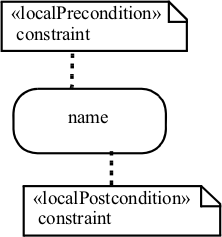
\includegraphics[scale=1]{./pics/local_postconditionsDiagram.PNG}
\end{figure}
\subsection{OCL}
\label{sec:OCL}


% \section{Taxonomy of Model Based Testing}
% Test Model,
% Unit Test,
% verdict,
% Test data,
% SUT,
% Harness/ stubs,
% declarative specification

